
\documentclass[12pt,a4paper]{article}



%Spacing Packages
\usepackage{fullpage}
\usepackage{a4wide}


%Other Packages
\usepackage{amssymb}
\usepackage{amsmath}
\usepackage{euscript}

\usepackage{graphicx}

\usepackage[lf]{venturis} %% lf option gives lining figures as default; 
			  %% remove option to get oldstyle figures as default
\usepackage[T1]{fontenc}


\begin{document}

\begin{quote}

\begin{center} {\large 24.118x -- Paradox and Infinity \\ \vspace{1mm}}
 {\large Problem Set 4: Omega Sequences \\ \vspace{1mm}}
 
\end{center}
\vspace{3mm}

\noindent How these problems will be graded:

\begin{itemize} 
\item Assessment will be based both on the arguments you give in support of your answers and on the answers themselves. There is no word limit.
\end{itemize} 

\end{quote}

\subsection*{Problems:}

\begin{enumerate}

\item Lazy wants to run from $A$ to $B$, but he likes to take breaks. He first stops halfway between $A$ and $B$ and takes a one-second break. He then stops halfway between \emph{that} point and $B$ and takes another one-second break, and so on. Is there a positive integer $n$ such that after $n$ seconds Lazy has reached point $B$? Explain your answer.
	
\item You have a wheel with a radius of 1 meter. You draw a red line going from the centre of the wheel to the twelve o'clock position:
	
\begin{center}
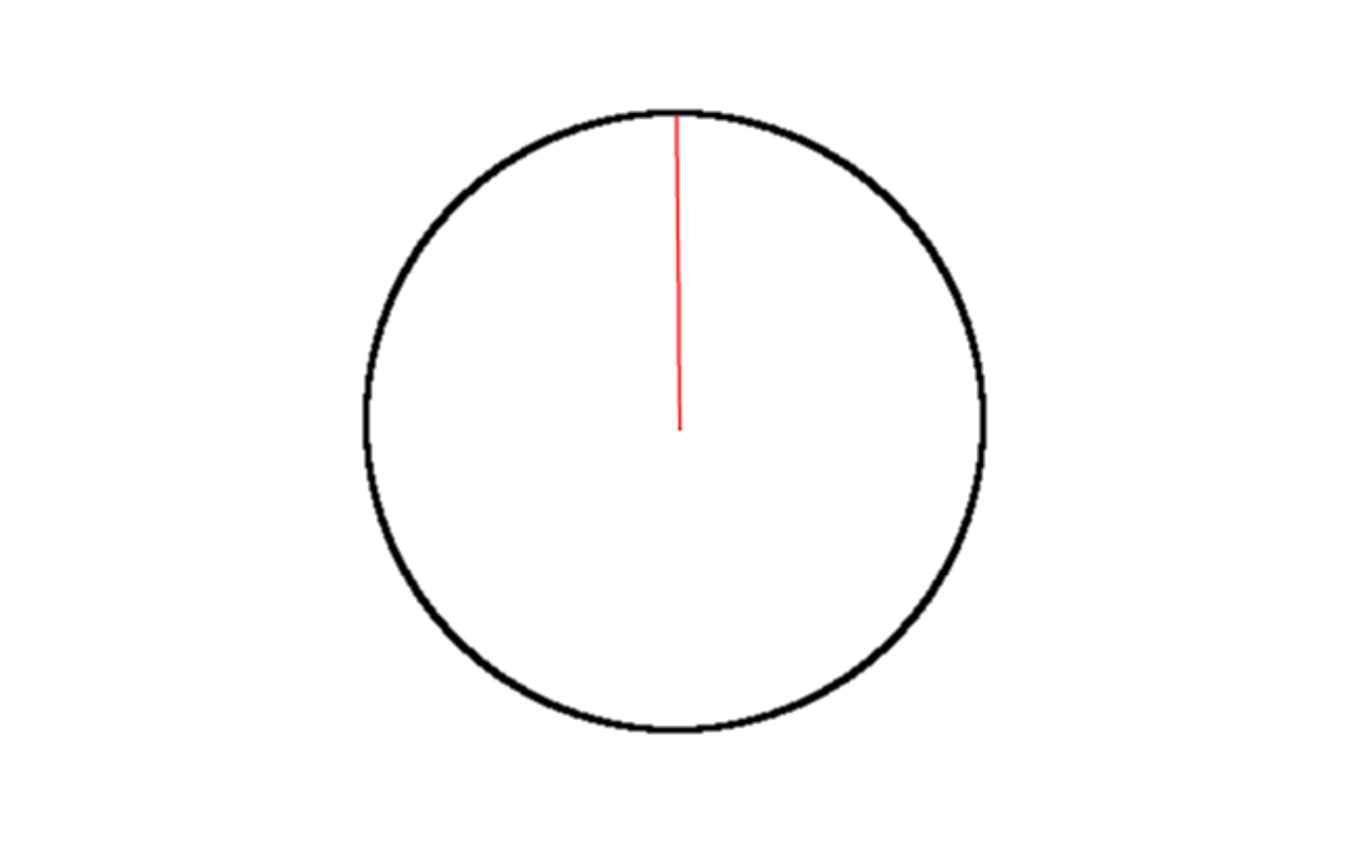
\includegraphics[scale=.2]{base}
\end{center}
	
	 You then rotate the wheel, in steps. At each step, you rotate the wheel one radian clockwise, so that the outermost point of the red line travels 1 meter around the perimeter of the wheel. Here is the first rotation:
	
	\begin{center}
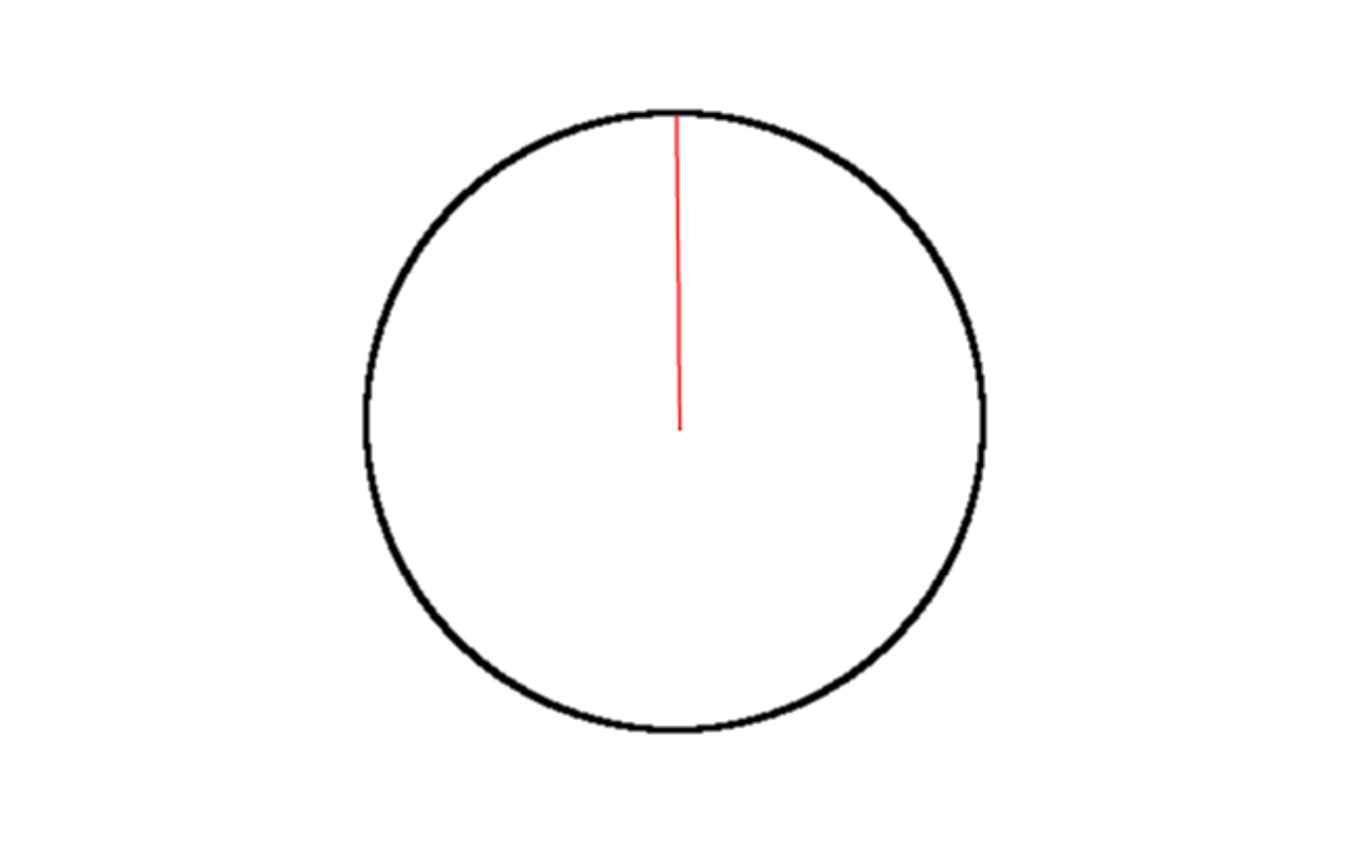
\includegraphics[scale=.2]{base}  \raisebox{13mm}{$\longrightarrow$} 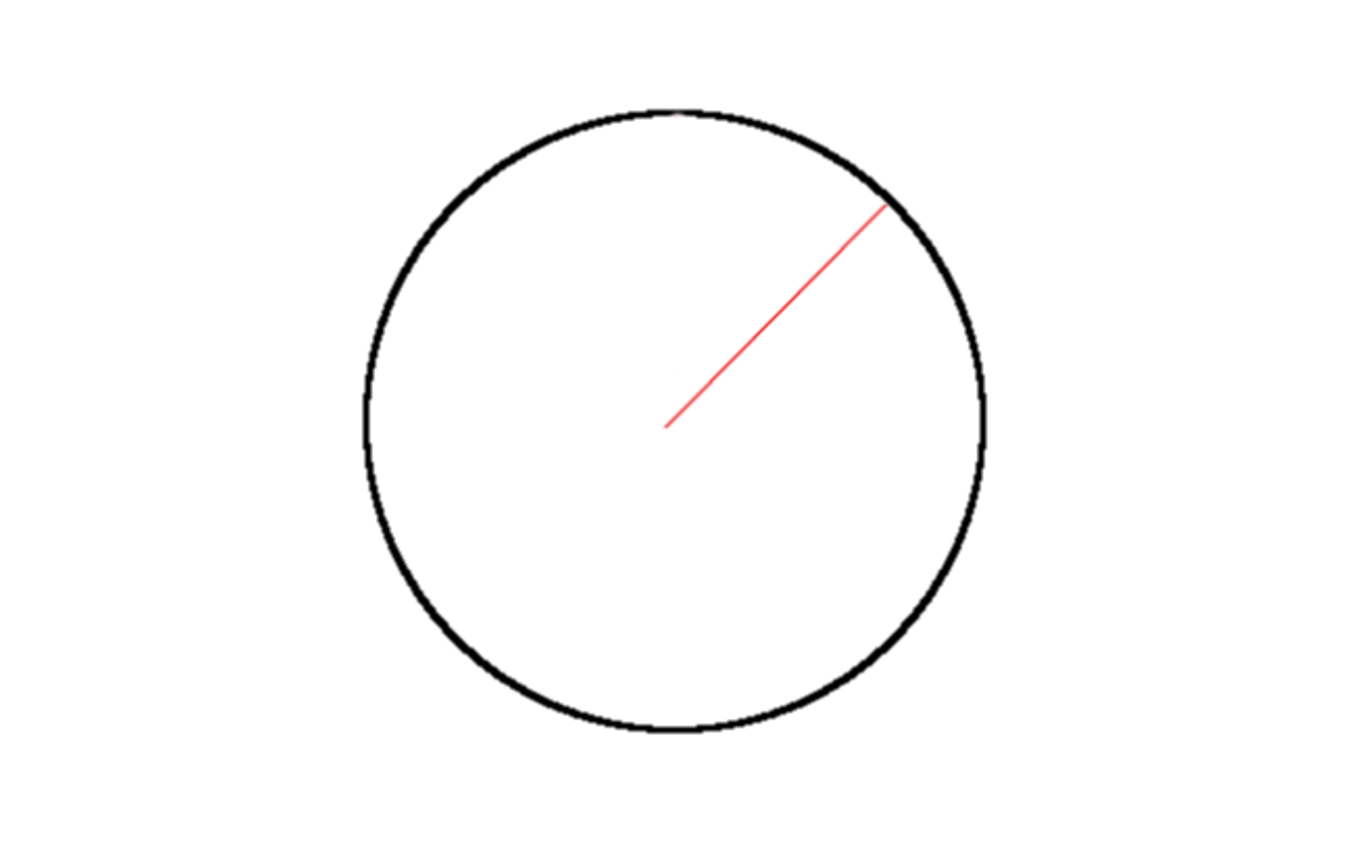
\includegraphics[scale=.2]{1rad}
\end{center}
Because the tip of the red line travels 1 meter around the perimeter after each rotation, and because the perimeter of the wheel is $2\pi$ meters (which is an irrational number of meters), there is no positive integer $n$ such that, after $n$ steps, the red line returns to a position it had occupied before.

Suppose you perform this operation infinitely many times, once for each positive integer. At 11:00am the red line is at the twelve o'clock position. At 11:30 you rotate the wheel one radian clockwise. At 11:45 you rotate the wheel another radian clockwise. And so forth: for each $n \geq 1$, you perform the $n$th rotation $\frac{1}{2^n}$ hours before noon. (We may assume that you perform rotations faster and faster, so that you always finish the previous rotation well before then next one is to take place.) You are done at noon.

Consider the following argument:

\begin{quote}
There is no $n>0$ such that, after $n$ steps, the red line returns to the twelve o'clock position. So, at noon, the red line can not be in the twelve o'clock position.
\end{quote}

Is this a valid argument? Explain your answer.

\item Consider a variant of the case in question 2. As before, you start by drawing a red line from the centre of the wheel to the twelve o'clock position. But this time you don't rotate the wheel. Instead, at each step you draw a red line at a one radian angle from the last line you drew. Here are the first two steps of the process:


	\begin{center}
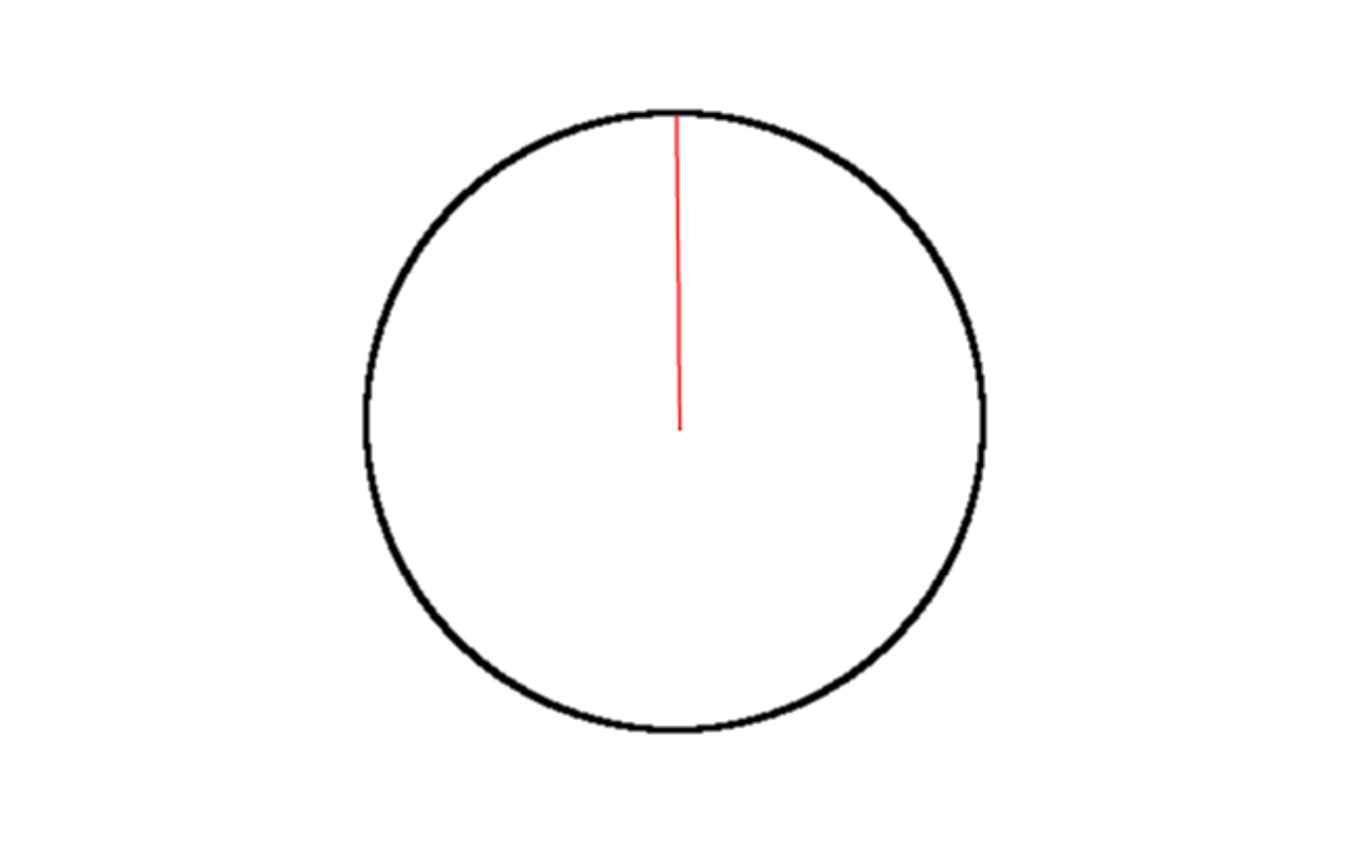
\includegraphics[scale=.2]{base}  \raisebox{13mm}{$\longrightarrow$} 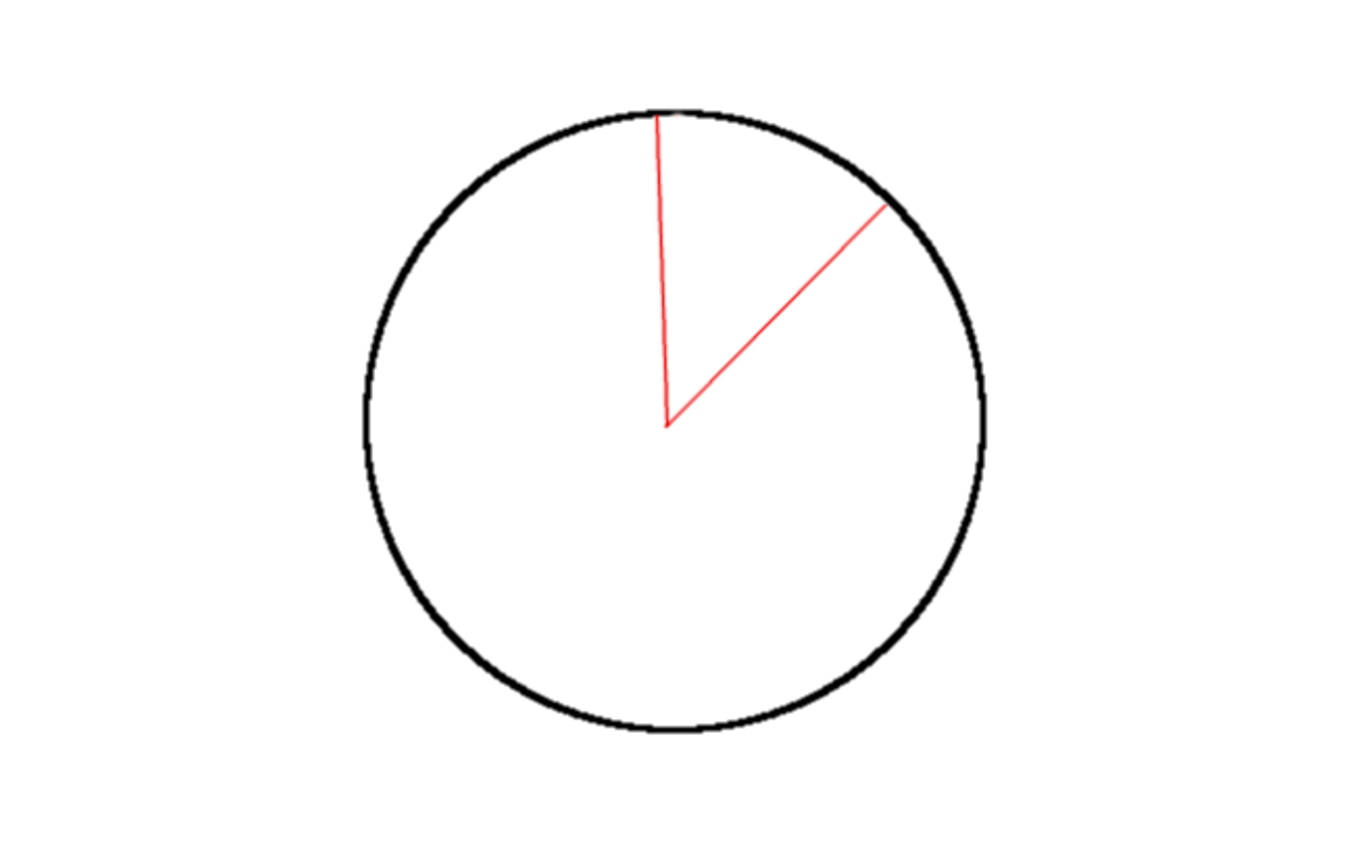
\includegraphics[scale=.2]{2rad}
\end{center}
You perform this operation infinitely many times, once for each natural number. At 11:00am you draw the initial red line, which we'll call ``line 0'', pointing to the twelve o'clock position, which we'll call ``position 0''. At 11:30 you draw an additional line, which we'll call ``line 1'', a radian away in the clockwise direction -- i.e., in the position we'll call ``position 1''. At 11:45 you draw line 2, a further radian away in the clockwise direction, which is position 2. And so forth: you draw line $n$ at $\frac{1}{2^n}$ hours before noon, and you draw it in position $n$, which is $n$ radians clockwise of position 0.

There is a well defined fact of the matter about what the wheel will look like from noon onwards. Namely: a radial line $r$ will be coloured red if and only if, for some natural number $n$, $r$ is exactly $n$ radians away from position 0, going clockwise.

Now it's afternoon, and you're done drawing lines on the wheel. It's time to start rotating!

Consider the result of rotating the wheel one radian in the clockwise direction. Each line $n$ will then occupy the position that line $n+1$ used to occupy --- so line 0 will occupy position 1, line 1 will occupy position 2, line 2 will occupy position 3, and so forth.

What about position 0? Will position 0 have a red line in it, or will it be blank? If you think about it, you'll see that position 0 must be blank, after one rotation clockwise, as, before rotation, one radian to the left of position 0 had to be blank. (Why? It has to do with the fact that $\pi$ is irrational. If you want to have this explained, ask me or one of the TAs about it.)

So, after rotating the wheel clockwise by one radian, the wheel will look exactly the way the unrotated wheel would have looked if you had skipped drawing line 0. 

Now suppose you rotate the wheel clockwise by one further radian. Each line $n$ will then occupy the position that, originally, line $n+2$ occupied. So line 0 will now be in position 2, line 1 in position 3, line 2 in position 4, and so forth. The blank at position 0 will now be in position 1. What about position 0? Again, it will be blank , for similar reasons to before. So after you rotate the wheel one radian further, for a total rotation of two radians, it'll look exactly the way the unrotated wheel would have looked if you had skipped drawing lines 0 and 1.

And so on. In general, after a total of $n$ rotations clockwise by a radian, the wheel will look exactly the way the original unrotated wheel would have looked if you had skipped drawing lines 0 through $n-1$.

Now: suppose that you rotate the wheel infinitely many times, once for each positive integer. At 1:30pm you rotate the wheel one radian in the clockwise direction. At 1:45 you rotate the wheel another radian in the clockwise direction, and so on; you are done by 2:00p.m.

Consider: what does the wheel look like at 2pm? Assuming that the wheel survives the process, and nothing else particularly weird happens, one of the following two arguments is sound:
\begin{quote}
\textbf{Argument 1}
After every rotation, every red line remains on the wheel. So, at 2 p.m., all the red lines are still on the wheel.
\end{quote}

\begin{quote}
\textbf{Argument 2}
For all $n$, position $n$ is blank after $n+1$ rotations, and remains blank. So at 2 p.m., position $n$ is blank for all $n$. And no rotation ever takes a red line to a radius other than position $n$, for some $n$. So at 2p.m. every non-position is also blank. So at 2p.m., the wheel is completely blank.
\end{quote}

Finally, here is your question: which of these two arguments is sound? What is wrong with the other argument?\footnote{I am told that the idea of this problem, and the previous one, comes originally from the young daughter of Oxford philosopher Frank Arntzenius (who wrote ``Infinity, Relativity and Smoothness'', linked from the syllabus).}

\item Fool has infinitely many dollar bills, and has labelled each of them with a different natural number (its ``serial number''). One minute before midnight, Fool gives you a dollar bill. Half a minute later, he gives you two dollars. Fifteen seconds later, he gives you four dollars. And so forth. (For each $i \geq 0$, Fool gives you $2^i$ dollars at $2^{-i}$ minutes before midnight.) There is, however, a catch. Each time you receive money from Fool, you are required to put together all your dollar bills, and burn the one with the lowest serial number. Assume that, at midnight, you have every dollar bill that you received from Fool and did not burn. How much money will you have at midnight? (Explain your answer.)
			
\item You have a dollar bill, and Fool has infinitely many. And, just as before, each bill has a serial number. 

One minute before midnight, you give Fool your dollar bill. Half a minute later, he gives you two dollars. Fifteen seconds later, you give him a dollar. Seven and a half seconds later, Fool gives you four dollars. And so forth. (For each $i \geq 0$, you give Fool one dollar at $2^{-2i}$ minutes before midnight and he gives you $2^{i+1}$ dollars at $2^{-(2i+1)}$ minutes before midnight.) Assume that, at midnight, you have every dollar bill that you received from Fool and did not return.

Question: is there a strategy you can follow, when it comes to giving dollar bills back to Fool, that maximises the amount of money you have at midnight? If so, describe such a strategy, and say how much money you have at midnight if you follow the strategy. If not, say why not, and say how much money you have at midnight.

\end{enumerate}



\end{document}

